\documentclass{bioinfo}
\copyrightyear{2017} \pubyear{2017}

\access{Advance Access Publication Date: Day Month Year}
\appnotes{Application Note}

\usepackage{url}

\begin{document}
\firstpage{1}

\subtitle{Subject Section}

\title[short Title]{Phylotyper: {\it In silico} predictor of molecular subtypes from gene sequences}
\author[Whiteside \textit{et~al}.]{Matthew D. Whiteside\,$^{\text{\sfb 1,}*}$, Chad R. Laing\,$^{\text{\sfb 1}}$ and Victor P.J. Gannon\,$^{\text{\sfb 1,}*}$}
\address{$^{\text{\sf 1}}$National Microbiology Laboratory, Public Health Agency of Canada, Lethbridge, AB, Canada, T1J 3Z4}

\corresp{$^\ast$To whom correspondence should be addressed.}

\history{Received on XXXXX; revised on XXXXX; accepted on XXXXX}

\editor{Associate Editor: XXXXXXX}

\abstract{\textbf{Summary:} Whole genome sequencing (WGS) is being adopted in public health for improved surveillance and outbreak analysis.
Molecular subtyping has been used in public health to infer phenotypes and flag high-risk bacterial strain groups.
\textit{In silico} tools that predict molecular subtypes from gene sequences are needed to transition historical data to WGS-based protocols.
Phylotyper is a novel solution for \textit{in silico} molecular subtype prediction from gene sequences.
Designed for incorporation into WGS pipelines, it is a general prediction tool that can be applied to most molecular subtype schemes.
Phylotyper uses phylogeny to model the evolution of the subtype and infer subtypes for unannotated sequences.
The phylogenic framework in Phylotyper improves accuracy, provides useful contextual feedback, and is more capable of identifying novel subtypes over approaches based solely on sequence similarity.\\
\textbf{Availability and Implementation:} Phylotyper is a python package. It is available from: \url{https://github.com/superphy/insilico-subtyping}.\\
\textbf{Contact:} \href{matthew.whiteside@phac-aspc.gc.ca}{matthew.whiteside@phac-aspc.gc.ca}\\
\textbf{Supplementary information:} Supplementary data are available at \textit{Bioinformatics}
online.}

\maketitle

\section{Introduction}

Whole-genome sequencing (WGS) is transforming the public health field by providing an efficient method for surveying bacterial populations.
The speed, discriminatory power and broad utility of WGS can improve surveillance and outbreak analysis.
Adoption of WGS in public health, however, requires transitioning of historical data with the new methods \citep{Jenkins2015}.
One of the workhorse methods in public health is molecular subtyping (such as serotyping).
As a surveillance tool, subtypes provide a clearcut designation that is typically used to distinguish taxonomic groups and infer phenotypes, for example, pathogens from non-pathogens.
A WGS-based approach to subtyping would have several benefits over current subtype systems; it would be faster, have improved discrimination and would be cheaper and easier to maintain\citep{Jenkins2015}.
Accordingly, new \textit{in silico} tools have been developed to predict subtypes from WGS data \citep{Joensen2015,Ingle2016,CARRILLO2016}.

Phylotyper is a novel \textit{in silico} predictor of subtypes from sequence data. 
Phylotyper is unique in that it builds a phylogenetic tree consisting of reference sequences with known subtype and the unknown query sequences to help inform subtype prediction. 
Using phylogenetic ancestral state reconstruction to assign the likelihood of each subtype to the tree branch points, Phylotyper assigns an unknown query sequence a subtype based on the extrapolated value from its ancestors in the tree.

\section{Implementation}

The core of Phylotyper is an ancestral state reconstruction (ASR) method that has been adapted for hidden state prediction.
In phylogenetic analysis, ancestral state reconstruction involves the prediction of traits of ancestors from existent descendants.
This methodology can be extended to also predict properties in a limited number of existing strains.

In Phylotyper, the \texttt{rerootingMethod} function from the phytools R package is used to perform the ASR \citep{Revell2011}.
This function calculates the maximum marginal likelihood for unknown tip nodes in a phylogenetic tree.
The likelihood reflects the most likely state for the node given the empirically estimated subtype evolution model and phylogeny.
In the context of Phylotyper, the marginal likelihood provides a confidence value associated with a predicted subtype.

Phylotyper is developed in python and R. 
The steps in the Phylotyper pipeline are: 
(1) Identify subtype gene loci in input genomes using BLAST \citep{Camacho2009}.
(2) Align input genes against a pre-aligned set of reference genes using MAFFT's \texttt{--add} feature \citep{Katoh2013}.
(3) If multiple loci are involved, concatenate individual alignments into superalignment.
(4) Generate maximum likelihood phylogenetic tree of aligned genes with FastTree \citep{Price2010}.
(5) Run phytools \texttt{rerootingMethod} using the phylogenetic tree and assigned subtypes \citep{Revell2011}.
(6) Identify the subtype with maximum marginal likelihood for the unknown genes and report to user in text output file.
Users are also provided with an image of the phylogenetic tree overlaid with the likelihood values (e.g. Figure~1\vphantom{\ref{fig:01}}).

\begin{figure}[!tpb]%figure1
\centerline{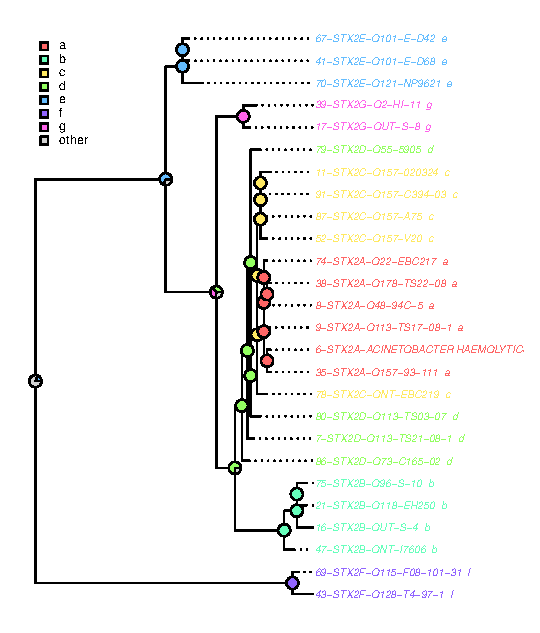
\includegraphics{fig01.eps}}
\caption{Phylogenetic tree for select Stx2 genes. 
The subtype marginal likelihood is displayed at each node as a pie chart.
The full Stx2 tree is displayed in Supplementary Figure S1.}\label{fig:01}
\end{figure}

Phylotyper was designed to be incorporated into a WGS workflow.  
The main input into Phylotyper is assembled genome sequences.  
Putative loci needed for the subtype scheme are identified in the input genomes using BLAST \citep{Camacho2009}.
The identified loci are then sent to the Phylotyper subtype prediction module.
It is possible in Phylotyper to use multiple loci for subtype prediction.
Individual loci alignments are concatenated to form a single superalignment that is used to build the phylogenetic tree.

Currently, subtype schemes for \emph{Escherichia coli} (\textit{E. coli}) are available in the Phylotyper package, and in addition to Stx include intimin and serotyping  (Supplementary Table~1).
However, the Phylotyper software aslo has the capability to add new subtype schemes. 
Creating a new subtype scheme will save the required reference files, allowing newly added schemes to be easily re-run from Phylotyper.
Checks are built-in to the new subtype pipeline to ensure the assumptions of the Phylotyper approach are not violated.  

\section{Results}

To compare the performance of Phylotyper to a sequence similarity-based approach, we ran a leave-one-out cross validation analysis.
For this assessment, we developed a mock sequence-similarity based tool that assigns putative subtypes using BLAST.
The leave-one-out analysis examined the four subtype schemes available in Phylotyper. The results of the analysis indicated that the precision of the Phylotyper method is consistently higher than a top-BLAST hit approach (Supplementary Table S2).

\section{Discussion}

From assembled WGS data, Phylotyper can assign unclassifed strains a molecular subtype.
Currently the Phylotyper software offers subtyping schemes for \textit{E. coli}.
It can, however, be applied to most molecular subtype schemes and Phylotyper includes functionality to build new schemes.

Performance testing showed that Phylotyper is more robust than an approach based solely on sequence similarity.
Phylotyper computes an empirical model of subtype evolution to predict subtypes for unclassified sequences.
By estimating the phylogenetic distribution of each subtype, Phylotyper can more easily identify a novel subtype or accurately classify a novel sequence allele.
The phylogenetic framework in Phylotyper provides a statistical likelihood for interpreting novel alleles.
In comparison, the performance of a sequence similarity approach is highly dependent on the reference database.
This type of approach, there is no inherient mechanism to identify novel alleles.

Subtypes are mainly used as a proxy for evolutionarily-related bacterial strain groups or to infer phenotypes.
Recent analysis of serotype data revealed several inconsistencies between molecular subtype and genomic data \citep{DebRoy2016}.
Subtypes predicted using a phylogenetic framework is more consistent with the main uses of subtype information, so 
Phylotyper is uniquely capable to transition historical subtype data to new WGS systems.\vspace*{-10pt}

\section*{Funding}

This work is funded in part by the Public Health Agency of Canada and a grant from the Genomics Research and Development Initiative\vspace*{-12pt}

\bibliographystyle{natbib}

\bibliography{phylotyper}


\end{document}
